\chapter{Design of a Practical Encryption Scheme for Online Social Networks}
\label{cha:n}

\section{Online Social Network}
OSNs are getting more and more aware of the rising privacy concerns among their users. Therefore, most OSN services like Google+ and Facebook try to offer preferences that allow the user to determine their privacy up to a certain extent. In practice, most OSNs realise this by offering user specified groups of friends that can be selected when broadcasting a message. The OSN provider then ensures that the broadcasted message is only available to members inside the user specified group. However, these methods are insufficient for most privacy aware users.

\subsection{Definition}
The most commonly accepted definition of an \textit{Online Social Network} (OSN) in literature is from Boyd et al.~\cite{art:BoydE08}. However, since this definition is still too generic for the remainder of this text a slightly modified version is presented here.

\begin{defn}[Online Social Network~\cite{art:BoydE08}]
\label{def:osn_boyd}
 An \textit{online social network} (OSN) is a web-based service that allows individuals to:
 \begin{enumerate}
  \item Construct a public or semi-public profile within a bounded system
  \item Articulate a list of other users with whom they share a connection.
  \item View and traverse their list of connections and those made by others within the system
  \item Distribute messages to anyone visiting the system, any user of the system or subsets thereof 
  \setcounter{enumTemp}{\theenumi}
 \end{enumerate}
\end{defn}


\subsection{Model of Current OSN Situation}
\label{sec:model}
\begin{defn}[OSN user]
\label{def:user}
 An \textit{OSN user} $U$ is any entity that has a profile on the OSN and thus identifiable by a unique identifier \id{U}. The set containing all users of an OSN is denoted $\mathcal{U}$.
\end{defn}

An OSN user can perform different activities within the infrastructure of the OSN. Depending on the performed activity, the user is labeled as one of three different roles: a sender, a friend or a recipient.

\begin{defn}[Sender]
\label{def:sender}
 A \textit{sender} $A$ is an OSN user who broadcasts a message $m$ over the OSN infrastructure to varying subsets of OSN users, called the \textit{intended recipient set} $\mathcal{S}$, such that $\mathcal{S} \subseteq \mathcal{U}$.
\end{defn}

\begin{defn}[Intended recipient]
\label{def:recipient}
 An \textit{intended recipient} of a message $m$ is an OSN user who is explicitly designated by a sender $A$ to be part of the intended recipient set $\mathcal{S}$ of that message $m$. The intended recipient set $\mathcal{S}$ takes the form of a list of \id{}'s uniquely identifying other users' profiles in the OSN infrastructure.
\end{defn}

\begin{defn}[Friend]
\label{def:friend}
 An OSN user who shares a connection with another OSN user $U$ in the OSN infrastructure, is called a \textit{friend of the user $U$}. The set of all friends associated to a user $U$ is denoted $\mathcal{F}_U$, such that $\mathcal{F}_U \subseteq \mathcal{U}$.
\end{defn}

Currently, other entities than OSN's users $U \in \mathcal{U}$ associated with a profile $\id{U}$, can access the OSN services as well. If abstraction is made of entities with access to specific content, it suffices to define a set of \textit{viewers}.

\begin{defn}[Viewer]
\label{def:viewer}
 Any entity that is given access to the OSN belongs to the set of viewers $\mathcal{V}$. All viewers with access to non-public content of a profile $\id{U}$ of a user $U$ are in the set $\mathcal{V}_U \subseteq \mathcal{V}$.
\end{defn}

Many different entities can be part of the set $\mathcal{V}$, e.g. OSN users, advertising companies, system administrators of the OSN or software applications specifically developed for the OSN. Usually, the OSN determines who is part of $\mathcal{V}$. Therefore, a user $U$ often has no control in who is a member of $\mathcal{V}_U$.

Following the example illustrated by Figure~\ref{fig:current_model}, Sender $A$ wants to broadcast a message $m$ over the OSN infrastructure to the intended recipient set $\mathcal{S}$. As $A$ only wants to share the message with a specific group of friends, $A$ defines the intended recipient set, such that $\mathcal{S} \subset \mathcal{F}_B$. Next, $A$ sends $m$ to the OSN's distribution server along with the intended recipient set $\mathcal{S}$. The OSN Server further distributes the message to all users in $\mathcal{S}$. Also a subset of third party applications and advertisers get access to the distributed message if they are inside the viewers group $\mathcal{V}_B$. Every entity who has access to the message is coloured blue in Figure~\ref{fig:current_model}.

Figure~\ref{fig:current_model} illustrates previous definitions applied to an OSN as it is often encountered on the internet. The different sets in Figure~\ref{fig:current_model} are defined as follows:
\begin{itemize}
 \item The intended recipient set,
 \begin{equation*}
  \mathcal{S} = \{ \textrm{Recipient 1}, \textrm{Recipient 2} \}
 \end{equation*}
 \item The set of friends of user $B$,
 \begin{equation*}
  \mathcal{F}_B = \{ \mathcal{S}, \textrm{Friend 1}, \textrm{Friend 2} \}
 \end{equation*}
 \item The set of viewers who have access to the profile of user $B$,
 \begin{equation*}
  \begin{split}
   \mathcal{V}_B = \{ \mathcal{F}_B, \textrm{Sender } A, \textrm{Advertiser 1}, \textrm{Application 1} \}
  \end{split}
 \end{equation*}
 \item The set of entities with access to the OSN,
\begin{equation*}
\begin{split}
 \mathcal{V} = \{ \mathcal{V}_B, \textrm{User 1}, \textrm{User 2}, \textrm{Advertiser 2}, \textrm{Application 2} \}
\end{split}
\end{equation*}
\item The set of all users in the OSN,
\begin{equation*}
 \mathcal{U} = \{ \mathcal{F}_B, \textrm{Sender} A, \textrm{User 1}, \textrm{User 2}\}
\end{equation*}
\end{itemize}


\begin{figure}
    \begin{center}
    \scalebox{0.78}{
        \begin{tikzpicture}[auto, node distance=-2mm, align=center,
            block/.style={rectangle,text width=6em,text centered,minimum height=9mm},
            line/.style={draw,very thick, ->},
            line2/.style={draw,very thick, <->},
            leg/.style={text centered},
            ]
            % Recipient set polygon
            \draw[dashed,color=cyan] (3.5,4) -- (8.5,4) -- (8.5,1.75) -- (3.5,1.75) -- (3.5,4);
            % Friends polygon
            \draw[dashed] (3,4.5) -- (9,4.5) -- (9,-0.25) -- (3,-0.25) -- (3,4.5);
            % Viewers Polygon
            \draw[dashed] (-5,5) -- (9.5,5) -- (9.5,-0.75) -- (-5,-0.75) -- (-5,5);
            % OSN Polygon
            \draw[dashed] (-5.5,5.5) -- (10,5.5) -- (10,-2.75) -- (-5.5,-2.75) -- (-5.5,5.5);
            %\draw[help lines] (-6,-5) grid (8,6);
            \path
                % Images
                (0,3) node [block] (pkg) {
\includegraphics[scale=0.15]{img/bluepkg.png}}
                (-4,3) node [block] (alice) {
\includegraphics[scale=0.15]{img/bluealice.png}}
                (5,3) node [block] (bob) {
\includegraphics[scale=0.15]{img/bluebob.png}}
                (7,3) node [block] (bob1) {
\includegraphics[scale=0.15]{img/bluebob.png}}
                (5,1) node [block] (bob2) {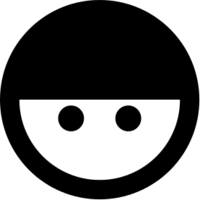
\includegraphics[scale=0.15]{img/bob.png}}
                (7,1) node [block] (alice1) {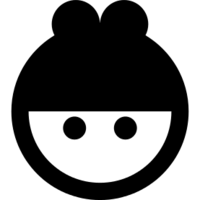
\includegraphics[scale=0.15]{img/alice.png}}
                (-1.5,1) node [block] (adv) {
\includegraphics[scale=0.15]{img/bluemoneyman.png}}
                (1.5,1) node [block] (app) {
\includegraphics[scale=0.15]{img/blueapp.png}}
                
                (1.5,-1.5) node [block] (app2) {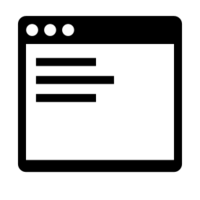
\includegraphics[scale=0.15]{img/app.png}}
                (-1.5,-1.5) node [block] (adv2) {
\includegraphics[scale=0.15]{img/moneyman.png}}
                
                
                (5,-1.5) node [block] (alice2) {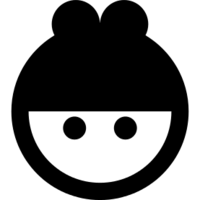
\includegraphics[scale=0.15]{img/alice.png}}
                (7,-1.5) node [block] (bob3) {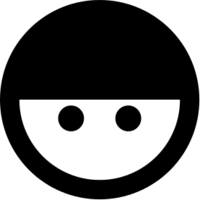
\includegraphics[scale=0.15]{img/bob.png}}
                
                (-1.5,-4) node [block] (spy1) {
\includegraphics[scale=0.15]{img/spy.png}}
                (1.5,-4) node [block] (spy2) {
\includegraphics[scale=0.15]{img/spy.png}}
                % Text
                (0,5.5) node [leg,fill=white] (white_block) {Entities with access to the OSN $\mathcal{V}$}
                (0,5) node [leg,fill=white] (white_block) {Entities with access to $B$'s Profile $\mathcal{V}_B$}
                (6,4) node [color=cyan,leg,fill=white] (white_block) {Intended Recipient Set $\mathcal{S}$}
                (6,4.5) node [leg,fill=white] (white_block) {Friends Set $\mathcal{F}_B$}
                (-2,3.25) node [leg,color=cyan] (white_block) {$m, \mathcal{S}$}
                ;
                
       \node[node distance=2mm, above=of pkg,color=cyan] {\textbf{OSN Broadcast Server}};
       \node[below=of adv,color=cyan] {Advertiser 1};
       \node[below=of adv2] {Advertiser 2};
       \node[below=of app2] {Application 2};
       \node[below=of alice2] {User 1};
       \node[below=of bob3] {User 2};
       \node[below=of bob,color=cyan] {Recipient 1};
       \node[below=of bob1,color=cyan] {Recipient 2};
       \node[below=of bob2] {Friend 1};
       \node[below=of alice1] {Friend 2};
       \node[below=of app2] {Application 2};
       \node[below=of alice,color=cyan] {Sender $A$};
       \node[below=of app,color=cyan] {Application 1};
       \node[node distance=-6mm,below=of spy1] {Outsider 1};
       \node[node distance=-6mm,below=of spy2] {Outsider 2};
       \begin{scope}[every path/.style=line,color=cyan]
        \path (alice.east) -- (pkg.west);
        %\path (pkg.south west) -- (adv.north);
        \path (-0.7, 2.3) -- (adv.north);
        \path (0.7,2.3) -- (app.north);
        \path (pkg.east) -- (3.5,3);
       \end{scope}


        \end{tikzpicture}
    }
    \end{center}
    \caption{Model of the current OSN situation. Entities with access to the message $m$ are coloured blue.}
    \label{fig:current_model}
\end{figure}

The OSN's infrastructure stores almost everything within the viewer set $\mathcal{V}$. The profiles of all users within the friends set $\mathcal{F}_B$, the list of \id{}'s within the intended recipient set $\mathcal{S}$, access rights of applications and advertisers that are part of $\mathcal{V}_B$ and access rights of entities within the set $\mathcal{V}$ are all explicitly stored somewhere on the servers of the OSN.

Note that not all OSNs support the functionality to define intended recipient sets $\mathcal{S}$ on a per message basis. In OSNs like Twitter the standard privacy settings are such that message are always published publicly. Therefore, the model from Figure~\ref{fig:current_model} only holds for a specific subset of OSNs like Facebook or Google+. More public OSNs like Twitter would require less sets of entities to model their behaviour.

It requires almost no additional effort to transform the model from Figure~\ref{fig:current_model} such that it also takes the sharing of other media than messages into account. The model could then adopted for use on SNSs like Youtube or Instagram as well. However, this falls out of the scope of this thesis.

\section{Issues with Current OSN Situation}
\label{sec:issues_with_current_osn_situation}
There are several issues with the current OSN situation as modelled in Figure~\ref{fig:current_model}.

First, there is a clear mismatch between the expectations of Sender $A$ and the functionality of the OSN. When a privacy-aware user like sender $A$ takes the effort to define an intended recipient set $\mathcal{S}$, she expects to have full control on who has access to her messages $m$. In reality, sender $A$ only has partial control since the OSN determines all other entities in $\mathcal{V}_A$ that are not part of sender $A$'s friend list $\mathcal{F}_A$. In some OSNs a user first has to give permission to third party applications before access is granted to the user's content. Note that this gives more control to OSN users on determining who is inside the viewers set $\mathcal{V}_B$. Nevertheless, in practice it is still hard to get a concise overview from the OSN on everyone inside $\mathcal{V}_B$.

Second, any user broadcasting messages over the OSN infrastructure has to trust the OSN that it effectively operates as claimed. If the OSN broadcast server in Figure~\ref{fig:current_model} would accidentally broadcast messages publicly despite of the sender's privacy settings, it would be hard for the Sender to find out.

Furthermore, the users of the OSN have to rely on the security of the OSN's infrastructure. If one of the outsiders in Figure~\ref{fig:current_model} would succeed in hacking the OSN's digital infrastructure, he would have immediate access to all sensible information stored on the OSN's servers. Similarly, governments can subpoena the OSN to disclose sensible information on certain users with the argument of national security.

Another significant point is that the OSN fully determines which access policies are supported. As already mentioned in Section~\ref{sec:model}, not all OSNs offer the definition of an intended recipient set on a per message basis. Even OSNs currently supporting this functionality can suddenly stop offering the service. Moreover, nothing prevents OSN providers from changing their privacy policy on a regular basis, thereby complicating users to define the access policy of their choice.

Besides the earlier mentioned issues, the OSN often operates with a corporate mentality. The OSN has no initiative to stop adding advertisers and applications to the set of entities with access to a user's profile $\mathcal{V}_B$. The more information advertising companies receive from the OSN provider, the better they can tailor advertisements to the user. The more third party applications rely on the OSNs infrastructure, the more appealing the OSN business model looks like. Therefore, OSNs have often no initiative to offer stricter access control policies to their users.

\section{Cryptographic Goals}
\label{sec:cryptographic_goals}
Section~\ref{sec:goals_of_this_thesis} already defined a set of abstract goals for an architecture trying to solve the current privacy issues in OSNs. These goals stated that a solution should be user friendly, applicable and immediately ready to use. Besides from these general design goals, it is now possible to define specific cryptographic requirements as well. A well-designed encryption scheme should be able to achieve the following cryptographic goals when publishing a message $m$ to a set of intended recipients $\mathcal{S}$ on an OSN with the help of an encryption scheme:
\begin{itemize}
 \item \textbf{Confidentiality:} The message is protected from disclosure to unauthorised parties, i.e. all entities that are not explicitly in the recipient set $\mathcal{S}$.
 \item \textbf{Outsider recipient anonymity:} The intended recipients of a broadcasted message should be anonymous to anyone not included in the intended recipient set $\mathcal{S}$. This implies that neither the OSN has to know who the recipients are. (Definition~\ref{def:outsider_anonymity} gives a more formal definition of outsider-anonymity).
 \item \textbf{No redundancy:} The message should be published only once to reach every recipient in the intended recipient set $\mathcal{S}$.
 \item \textbf{Authenticity:} The recipients of the message have reasonable assurances of the message's origin.
 \item \textbf{Integrity:} The recipients are assured the message is distributed in its original form as posted by the sender.
 \item \textbf{No key escrow:} Private keys are only disclosed to the owners of the public key. No other entity should be able to have more information on one's secret key in the information theoretic sense.
 \item \textbf{Key validation:} All users of the system should be able to verify the correctness of their private keys.
 \item \textbf{Limited key validity:} Private keys of users should only be valid for a limited period of time to limit the damage of potentially lost private keys.
\end{itemize}

\section{Design Decisions}
Our architecture is further developed by keeping the earlier mentioned cryptographic design goals in mind.

\label{sec:design_decisions}
\subsection{Confidentiality}
Confidentiality can be achieved by applying an encryption scheme before broadcasting a message. Current solutions like Scramble~\cite{art:BeatoKW11} and Persona~\cite{art:BadenBSBS09} rely on rather classic public key infrastructures thereby requiring the OSN user to subscribe to a third party key infrastructure. These key infrastructures are required to authenticate and store the public keys of all security aware users. However, this does not correspond to the general design goals from Section~\ref{sec:goals_of_this_thesis} stating that the proposed solution should be both user friendly and immediately ready to use.

Identity-based encryption (IBE) can be used to achieve both confidentiality and the general design goals of usability and applicability. During the design of our scheme, three IBE schemes were considered as a potential candidate: Boneh and Franklin IBE~\cite{art:BonehF01}, Sakai and Kasahara IBE~\cite{art:SakaiK03} and Gentry IBE~\cite{art:Gentry06}. For a more elaborate discussion on why only these schemes were considered, the reader is referred to Section~\ref{sec:evolution_of_be}.

Table~\ref{tab:ibe_security_comparison} lists the different security properties of all schemes. The Gentry IBE scheme has the highest security level since it is the only scheme proven secure in the standard model. In the random oracle model, Boneh and Franklin IBE is preferred over Sakai and Kasahara IBE since it relies on the BDH assumption which is more widely accepted than the stronger BDHI assumption.

The execution times of all considered IBE schemes are illustrated in Table~\ref{tab:ibe_performance_comparison}. Experiments were conducted on an Intel Core 2.4 GHz i5 processor with 8 Gb of 1600 MHz DDR3L onboard memory. Pairing computations were implemented using the multi-precision MIRACL library~\cite{art:Scott03}. The Gentry IBE scheme was first transformed to the asymmetric setting to give a fair basis of comparison. The exact transformed Gentry IBE scheme is depicted in Appendix~\ref{app:gentrys_ibe_scheme}. 

Table~\ref{tab:ibe_performance_comparison} clearly illustrates the price there is to pay for security in the standard model. Therefore, Boneh and Franklin IBE was chosen as the preferred IBE scheme despite the dependency on the random oracle assumption.


\begin{table}
  \centering
  \begin{tabular}{@{}lccr@{}} \toprule
    \multicolumn{3}{r}{Security Proof} \\ \cmidrule(r){2-4}
    IBE Scheme    & IND-ANO-CCA & Standard model & Assumption \\ \midrule
    Boneh and Franklin & \Checkmark & \XSolidBrush  & BDH \\
    Sakai and Kasahara & \Checkmark & \XSolidBrush & BDHI \\
    Gentry & \Checkmark & \Checkmark & q-BDHE \\ \bottomrule
  \end{tabular}
  \caption{Security comparison of considered IBE schemes}
  \label{tab:ibe_security_comparison}
\end{table}

\begin{table}
  \centering
  \begin{tabular}{@{}lrrrr@{}} \toprule
    \multicolumn{4}{r}{Execution time (ms)} \\ \cmidrule(r){2-5}
    IBE Scheme    & IBE.Setup & IBE.Extract & IBE.Encrypt & IBE.Decrypt \\ \midrule
    Boneh and Franklin & 368.10 & 13.84 & 271.90 & 252.82 \\
    Sakai and Kasahara & 1257.72 & 20.49 & 319.83 & 259.17\\
    Gentry & 24.49 & 37.46 & 1136.65 & 911.32 \\ \bottomrule
  \end{tabular}
  \caption{Performance comparison of considered IBE schemes in MIRACL}
  \label{tab:ibe_performance_comparison}
\end{table}

IBE requires that OSN profiles can be uniquely identified by a unique public identifier \id{}. However, the decision on which string to use as identifier is highly dependent on the underlying OSN and therefore implementation dependent.

\subsection{Outsider Recipient Anonymity}
The outsider anonymity requirement from Section~\ref{sec:cryptographic_goals} is imposed on the recipient set since our solution is developed in the context of OSNs where user interaction plays an important role. Therefore, it is useful that members of the intended recipient set $\mathcal{S}$ know each other. For example, suppose that Alice broadcasts an encrypted message intended to Bob and Dylan using a scheme that fully hides the identity of the recipients. This implies that $\id{Bob}, \id{Dylan} \in \mathcal{S}$. As a reaction to Alice's message, Bob wants to write a reply to start a discussion. However, as Bob does not know which other users are allowed to see Alice's message, he can now only encrypt his reply to Alice thereby preventing Dylan from joining the discussion. Nevertheless, this discussion could have been useful to Dylan as well because otherwise Alice would not have included Dylan as a recipient in $\mathcal{S}$ in the first place.

From the outsider-anonymity requirement, it immediately follows that users not necessarily need to be friends to receive each other's messages. In the specific example of Alice, Bob and Dylan, it could be that Bob and Dylan both have Alice as a common friend while no immediate friend connection exists between Bob and Dylan. This should be taken into consideration when determining the identifiers of Bob's and Dylan's profiles, $\id{Bob}$ and $\id{Dylan}$ respectively.

As discussed in Section~\ref{sec:anobe}, broadcast encryption schemes can be made more efficient if the recipient set $\mathcal{S}$ is public. So if user interaction is really that important, why not make the intended recipient set public? Consider the example in which Bob's girlfriend celebrates her birthday in a few weeks. When Bob's girlfriend notices that Bob broadcasted an encrypted message to all her friends without including her as a recipient, she will probably know Bob is up to something. This is just one example of possible many that illustrates the negative impact on security, broadcasting of the recipient set $\mathcal{S}$ can have on real life situations. Depending on the context, information can be deduced about the message without decrypting it to plain text.

\subsection{No redundancy}
From the no redundancy requirement it immediately follows that a broadcast encryption scheme should be used, preferably one that hides the anonymity of recipients in the intended recipient set $\mathcal{S}$ to the outside world. However, apart from the outsider-anonymous broadcast encryption scheme from Fazio and Perera~\cite{art:FazioP12}, no efficient schemes of this kind are described in literature. Since the BE scheme from Fazio and Perera does not fully benefit from the advantages of IBE, the ANOBE scheme from Libert et al.~\cite{art:LibertPQ12} is preferred for further implementation. Since recipients still have to know who else is included in $\mathcal{S}$, the list of \id{}s within $\mathcal{S}$ is concatenated to the plaintext message before encryption.

The scheme from Libert et al. also offers non-repudiation by using signature schemes. Note however, that a trusted authority authorising and publishing the public keys is required for the implementation of signature schemes. Because the general design goals were applicability and user friendliness, no third party PKI can be supported. Therefore, the implemented scheme does not rely on signatures as in the original proposal from Libert et al.~\cite{art:LibertPQ12}.

If the security parameter is chosen to be $\lambda$, the IBE scheme in Algorithm~\ref{alg:full_indent} can only encrypt messages with a maximum length of $l$ bits. This can be seen since in the last step of \texttt{IBE.Encrypt} the message $m$ is encrypted by an XOR operation with the result of a hash function $H_3: \{ 0,1 \}^l \rightarrow \{ 0,1 \}^l$. Because asymmetric IBE schemes can only encrypt these fixed length messages, the scheme from Libert et al.~\cite{art:LibertPQ12} is altered such that the ciphertext in the original proposal contains a with IBE encrypted symmetric session key $k$ that is the same for each user in the recipient set $\mathcal{S}$ on a per message basis. The actual plaintext is then encrypted with a symmetric encryption scheme based on a mode of operation to support longer message lengths.

\subsection{Authenticity and Integrity}
\label{sec:authenticity_and_integrity}
Authenticity and integrity can be achieved at the same time by relying on an authenticated encryption scheme. The integrity of a message is then as strong as the security guarantees of the authenticated encryption scheme. 

Note however, that the authentication mechanism still relies on the security guarantees of the OSN. Since no third party PKI mechanism is used, there is no trusted party verifying the identity corresponding to a public key. In OSNs this is not an issue if IBE is used with unique profile identifiers as a public key. Consequently, such an IBE scheme ensures that messages encrypted under a public identifier can only be seen by the owner of the corresponding OSN profile. Verifying whoever owns the OSN profile remains the responsibility of the OSN and the judgement of the OSN profile's connections. However, if the authentication mechanism of the OSN is inadequate, anyone could login to a user's profile to impersonate the actual owner of the profile. Therefore, our proposed solution can not be more secure than the authentication mechanism of the OSN.

In more traditional communication schemes, authenticated encryption uses the symmetric key as agreed during an authenticated key agreement protocol like the Station-to-Station protocol~\cite{art:DiffieOW92}. Authenticity of ciphertexts generated by the authenticated encryption scheme than immediately follows from the usage of the same symmetric session key $k$ as earlier agreed during the protocol. However, since in the proposed solution every OSN user should be able to immediately broadcast confidential messages to other users of the OSN, no key agreement protocols will be used. With the publication of only one broadcast ciphertext, every user in the intended recipient set $\mathcal{S}$ should be immediately able to decrypt it to the original plaintext message $m$. Therefore, there is no real authenticity in the value of the tag $t$ generated by the authenticated encryption scheme because anyone with access to the user's profile could have chosen a random symmetric session key $k$ and have used it as an input to the authenticated encryption scheme. Unless, the only one with access to the user's profile is the actual owner of the profile. Therefore, the authenticity guaranteed by the authenticated encryption scheme boils down to the security of the authentication mechanism as powered by the OSN.


\subsection{No Key Escrow and Key Validation}
One of the major drawbacks of IBE schemes is that they inherently imply key escrow (Section~\ref{sec:pros_and_cons_of_ibe}). To circumvent the key escrow property of IBE schemes, multiple PKGs can be used implementing a distributed key generation (DKG) mechanism for IBE. Users can then verify their private keys by relying on the basics of commitment schemes (Section~\ref{sec:commitment_schemes}).

For the exact details on how a commitment scheme can achieve this verification mechanism, the reader is immediately referred to the exact proposed scheme in Section~\ref{sec:proposed_scheme}.

\subsection{Limited Key Validity}
IBE schemes do not allow revocation of public keys (Section~\ref{sec:pros_and_cons_of_ibe}). A solution to circumvent this drawback is by concatenating an expiration date to all public identifiers \id{}. However, these expiration dates should be publicly available to all OSN users since they are part of the public IBE key. To avoid the management of a third party infrastructure keeping track of expiration dates of all users, a special type of function could be used mapping identifiers \id{} to dates. An example of such a function is shown in Algorithm~\ref{alg:map_to_date}.

Algorithm~\ref{alg:map_to_date} is constructed such that step 1 to 4 only need to be executed once. The sender then stores values $d_1, h_1, m_1$ locally and only repeats step 5 for each recipient of the message. The exact implementation details could be hidden from the user in software. Different variants of Algorithm~\ref{alg:map_to_date} could be applied as well. The most important aspect is that everyone in the system uses the same function to map strings to expiration dates.

\begin{algorithm}
\caption{A function mapping strings to dates}
\label{alg:map_to_date}
\begin{description}
 \item \textbf{Goal}: Avoid a third party infrastructure that keeps track of expiration dates of key pairs in an IBE system
 
 \item \textbf{Result}: On input of a public identifier \id{} the algorithm returns an expiration date in the form \texttt{d/M/y h:m}.
\end{description}
 \begin{enumerate}
  \item Choose a hash function $H: \{ 0, 1 \}^* \rightarrow \{ 0,1 \}^l$ mapping binary strings of arbitrary length to binary strings of a fixed length $l$.
  \item Calculate $r = H \left( \id{} \right)$ and interpret the result $r$ as an integer.
  \item Calculate $tot_m = r \bmod 40320 = r \bmod \left( 60 \cdot 24 \cdot 28 \right)$, where $tot_m$ denotes the expiration time in minutes within a certain month.
  \item Calculate three integers $d_1, h_1, m_1$ denoting an expiration day, hour and minute respectively with $1 \leq d_1 \leq 28$, $0 \leq h_1 \leq 23, 0 \leq m_1 \leq 59$ as follows 
  \begin{enumerate}
   \item The expiration minute is calculated as $m_1 = tot_m \bmod 60$
   \item The expiration hour is calculated as $h_1 = \frac{tot_m}{60} \bmod 24$
   \item The expiration day is calculated as $d_1 = \frac{tot_m}{60 \cdot 24}$
  \end{enumerate}
  It can be shown that $d_1, h_1, m_1$ are chosen uniformly random within their boundaries if the random oracle assumption holds for the hash function $H \left( \cdot \right)$.
  \item Let \texttt{nowIsEarlierThan($d_1$,$h_1$,$m_1$)} be a function that returns \texttt{true} if the current time \texttt{d/M/y h:m} is before \texttt{$d_1$/M/y $h_1$:$m_1$} and \texttt{false} otherwise. Output the expiration date as
  \begin{enumerate}
   \item If \texttt{nowIsEarlierThan($d_1$,$h_1$,$m_1$)} = \texttt{true}, return \texttt{$d_1$/M/y $h_1$:$m_1$}.
   \item If \texttt{nowIsEarlierThan($d_1$,$h_1$,$m_1$)} = \texttt{false} and \texttt{M}$+1 \leq 12$, return \texttt{$d_1$/M/y $h_1$:$m_1$}.
   \item Else return \texttt{$d_1$/1/(y+1) $h_1$:$m_1$}
  \end{enumerate}
 \end{enumerate}
\end{algorithm}


\section{Security Model}
To achieve the design decisions from Section~\ref{sec:design_decisions}, the model from Figure~\ref{fig:current_model} changes significantly. Therefore, a group of PKGs is introduced in the original model with their own responsibilities.

\subsection{Model}
Distributed key generators (DKGs) were already discussed in depth in Section~\ref{sec:distributed_key_generation}. However, for the sake of completeness it is useful to introduce a DKG as an additional entity in the current OSN model to the ones already described in Section~\ref{sec:model}.

\begin{defn}[PKG in our security model]
\label{def:dkg}
 A \textit{Public Key Generator} (PKG) is an entity in the security model that never colludes with any other entity in the model since its prime motivation is to improve the current security situation in OSNs.
\end{defn}

\begin{figure}[ht]
    \begin{center}
    \scalebox{0.78}{
        \begin{tikzpicture}[auto, node distance=-2mm, align=center,
            block/.style={rectangle,text width=6em,text centered,minimum height=9mm},
            line/.style={draw,very thick, ->},
            line2/.style={draw,very thick, <->},
            leg/.style={text centered},
            ]
            % Recipient set polygon
            \draw [color=cyan] (3.5,4) -- (8.5,4) -- (8.5,2) -- (3.5,2) -- (3.5,4);
            % Friends polygon
            \draw[dashed] (3,4.5) -- (9,4.5) -- (9,-0.25) -- (3,-0.25) -- (3,4.5);
            % Viewers Polygon
            \draw[dashed] (-5,5) -- (9.5,5) -- (9.5,-0.75) -- (-5,-0.75) -- (-5,5);
            % OSN Polygon
            \draw[dashed] (-5.5,5.5) -- (10,5.5) -- (10,-2.75) -- (-5.5,-2.75) -- (-5.5,5.5);
            %\draw[help lines] (-6,-5) grid (8,6);
            \path
                % Images
                (0,3) node [block] (pkg) {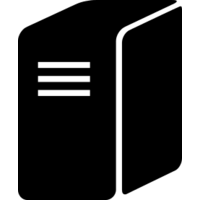
\includegraphics[scale=0.15]{img/pkg.png}}
                (-4,3) node [block] (alice) {
\includegraphics[scale=0.15]{img/bluealice.png}}
                (5,3.25) node [block] (bob) {
\includegraphics[scale=0.15]{img/bluebob.png}}
                (7,3.25) node [block] (bob1) {
\includegraphics[scale=0.15]{img/bluebob.png}}
                (5,1) node [block] (bob2) {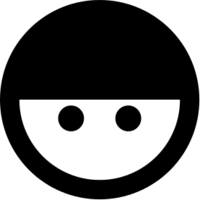
\includegraphics[scale=0.15]{img/bob.png}}
                (7,1) node [block] (alice1) {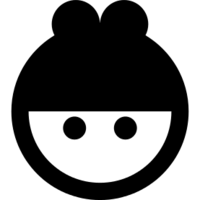
\includegraphics[scale=0.15]{img/alice.png}}
                (-1.5,1) node [block] (adv) {
\includegraphics[scale=0.15]{img/moneyman.png}}
                (1.5,1) node [block] (app) {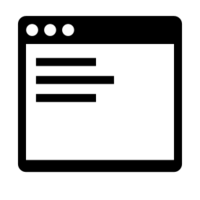
\includegraphics[scale=0.15]{img/app.png}}
                
                (1.5,-1.5) node [block] (app2) {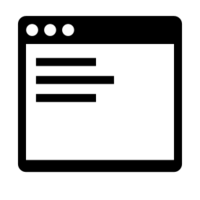
\includegraphics[scale=0.15]{img/app.png}}
                (-1.5,-1.5) node [block] (adv2) {
\includegraphics[scale=0.15]{img/moneyman.png}}
                
                % DKGs
                (-4,7) node [block] (pkg1) {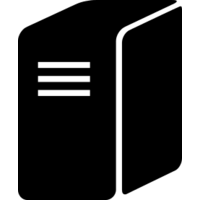
\includegraphics[scale=0.15]{img/pkg.png}}
                (0,7) node [block] (pkg2) {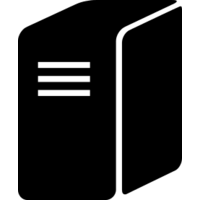
\includegraphics[scale=0.15]{img/pkg.png}}
                (4,7) node [block] (pkg3) {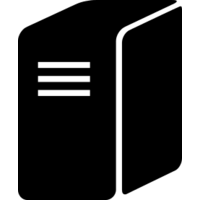
\includegraphics[scale=0.15]{img/pkg.png}}
                (8,7) node [block] (pkg4) {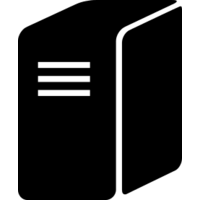
\includegraphics[scale=0.15]{img/pkg.png}}
                
                (5,-1.5) node [block] (alice2) {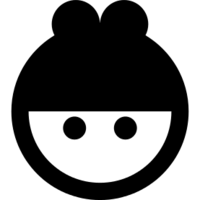
\includegraphics[scale=0.15]{img/alice.png}}
                (7,-1.5) node [block] (bob3) {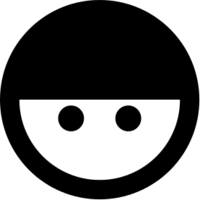
\includegraphics[scale=0.15]{img/bob.png}}
                
                (-1.5,-4) node [block] (spy1) {
\includegraphics[scale=0.15]{img/spy.png}}
                (1.5,-4) node [block] (spy2) {
\includegraphics[scale=0.15]{img/spy.png}}
                % Text
                (0,5.5) node [leg,fill=white] (white_block) {Entities with access to the OSN $\mathcal{V}$}
                (0,5) node [leg,fill=white] (white_block) {Entities with access to $B$'s Profile $\mathcal{V}_B$}
                (6,2) node [leg,fill=white] (white_block) {Intended Recipient Set $\mathcal{S}$}
                (6,-0.25) node [leg,fill=white] (white_block) {Friends Set $\mathcal{F}_B$}
                (-2,3.25) node [leg] (white_block) {$c$}
                ;
                
       \node[node distance=2mm, above=of pkg] {\textbf{OSN Broadcast Server}};
       \node[below=of adv] {Advertiser 1};
       \node[below=of adv2] {Advertiser 2};
       \node[below=of app2] {Application 2};
       \node[below=of alice2] {User 1};
       \node[below=of bob3] {User 2};
       \node[below=of bob,color=cyan] {Recipient 1};
       \node[below=of bob1,color=cyan] {Recipient 2};
       \node[below=of bob2] {Friend 1};
       \node[below=of alice1] {Friend 2};
       \node[below=of app2] {Application 2};
       \node[below=of alice,color=cyan] {Sender $A$};
       \node[below=of app] {Application 1};
       \node[below=of pkg1] {\textbf{PKG 1}};
       \node[below=of pkg2] {\textbf{PKG 2}};
       \node[below=of pkg3] {\textbf{PKG 3}};
       \node[below=of pkg4] {\textbf{PKG 4}};
       \node[node distance=-6mm,below=of spy1] {Outsider 1};
       \node[node distance=-6mm,below=of spy2] {Outsider 2};
       \begin{scope}[every path/.style=line]
        \path (alice.east) -- (pkg.west);
        %\path (pkg.south west) -- (adv.north);
        \path (pkg.east) -- (3,3);
        \path (-0.7, 2.3) -- (adv.north);
        \path (0.7,2.3) -- (app.north);
       \end{scope}
       \begin{scope}[every path/.style=line2]
        \path (4,6) -- (bob);
        \path (7.75,6) -- (bob);
        \path (8,6) -- (bob1);
        \path (4.25,6) -- (bob1);
       \end{scope}


        \end{tikzpicture}
    }
    \end{center}
    \caption{Model of the new OSN situation. Entities with the ability to decrypt the ciphertext are coloured blue.}
    \label{fig:new_model}
\end{figure}

Figure~\ref{fig:new_model} illustrates a variation on the original model of the OSN situation in Figure~\ref{fig:current_model}. At the top of Figure~\ref{fig:new_model} four PKGs are introduced implementing a $\left( t, n \right)$ DKG protcol (Section~\ref{sec:distributed_key_generation}) with $t = 2$ and $n = 4$. Double arrows represent the secure communication process in which the recipients communicate with the PKG to receive a share of their secret key. In Figure~\ref{fig:generic_ibe_scheme} this communication was illustrated by two separate single arrows between the PKG and Bob. However, abstraction is made of the exact communication protocol between the recipients and the PKG.

Apart from the newly introduced PKGs, there are some other rather subtile changes in Figure~\ref{fig:new_model} when compared to Figure~\ref{fig:current_model}. Sender $A$ no longer specifies the set of intended recipients $\mathcal{S}$ to the OSN broadcast server. Therefore, the OSN broadcast server delivers the message to all entities with access to $A$'s profile $\mathcal{V}_A$. Note that even Friend 1 and 2 are able to see the broadcasted message which was not the case in Figure~\ref{fig:current_model}. However, since the broadcasted message is actually a ciphertext $c$ of the original message $m$, only the entities in blue will be able to read the confidential content of the original plaintext message $m$.

\section{Threat Model}

\subsection{Adversary Definition}
We consider an adversary in the model illustrated in Figure~\ref{fig:new_model}, to be any computationally bounded entity trying to violate one or several of the following properties:
\begin{enumerate}
 \item \textbf{Confidentiality:} The entity tries to violate the confidentiality of encrypted messages, i.e. uncovering information within a broadcasted ciphertext. This can either be the intended recipient set $\mathcal{S}$ or the actual content of the plaintext message $m$.
 \item \textbf{Integrity:} The entity tries to violate the integrity of encrypted messages, i.e. changing the ciphertext $c$ or the plaintext $m$ such that it differs from the way it was originally drafted by the sender.
 \item \textbf{Availability:} Any entity apart from the original sender, tries to prevent messages from being broadcasted by bringing down parts of the architecture or the OSN. 
\end{enumerate}

\subsection{Assumptions on the PKG}
\label{sec:assymptions_on_pkg}
This thesis focusses mainly on the adoption of user friendly broadcast encryption in OSNs. Therefore, PKGs are considered to always behave as described in the DKG protocol. Note that this is a simplification of a PKG as it is often encountered in real-world applications. However, considering PKGs as malicious requires far more complex distributed key generation algorithms which are out of the scope of this thesis. For DKG protocols that can be used in more hostile PKG environments as encountered in practice, the reader is referred to Kate et al.~\cite{art:KateHG12}.

\subsection{Assumptions on the OSN}
OSNs are assumed not to violate integrity neither availability. Nothing can be done to prevent the OSN from actively altering its own resources to bring down the proposed IBE architecture. It can not be prevented that a user of IBE on the OSN infrastructure gets blocked by the OSN provider. Neither can it be prevented that OSNs delete messages because they are encrypted. OSNs can also easily impersonate the owner of a profile in their infrastructure. Therefore, from this moment onwards, OSNs are assumed to not act as an active adversary. It is assumed that as soon as privacy aware users notice this kind of OSN behaviour, they will adopt to more reliable OSN alternatives. However, our assumptions do not prevent the OSN from trying to passively break confidentiality as they have every motivation for it in the context of their current business model.

Another assumption on the OSNs infrastructure is that the authentication mechanism of the OSN is secure. This is primarily important for reasons as discussed in Section~\ref{sec:authenticity_and_integrity}.

These assumptions on the OSN are ideal assumptions that will probably hold as long as only the minority of the OSN users applies encryption mechanisms to their network. It is still unknown how OSNs will react if variations to the proposed encryption mechanism find common acceptance in their wide user base.

\subsection{Assumptions on the User}

In order to achieve a strong encryption mechanism, users are unlimited in their abilities to behave as an adversary. However, one subtle assumption is made on users that are part of $\mathcal{S}$. Users in $\mathcal{S}$ are assumed not to break their social contract. That is, if a sender broadcasts a confidential message to a selected set of recipients, the recipients are assumed not to decrypt the encrypted message and rebroadcast the confidential content to any entity not in the original recipient set. In fact, no existing encryption mechanism provides protection against such misbehaviour, although traitor tracing schemes~\cite{art:ChorFNP00} discourage users from treating by indicating who broke his social contract. However, for the remainder of this text intended recipients are assumed trustworthy in that they not break the social contract.
%Due to the proposed encryption mechanisms, the OSN provider storing the broadcasted ciphertext messages should not be able to derive more information than any other entity in the model. However, careless implementation of the proposed encryption mechanism could still give away more information to the OSN than desired.

%A sender should never use the privacy mechanisms provided by the OSN. If a sender $B$ specifies the intended recipient set $\mathcal{S}$ in the infrastructure of the OSN, the recipient set is obviously no longer private. In this case, both the OSN as well as other users within the set of entities with access to the senders profile $\mathcal{V}_B$ can possibly learn information on the recipients and the content of the message.




%%%%%%%%%%%%%%%%%%%%%%%%%%%%%%%%%%%%%
%% \subsection{Active Adversaries} %%
%%%%%%%%%%%%%%%%%%%%%%%%%%%%%%%%%%%%%

%Active adversaries try to alter system resources to affect their operation or actively take part in the protocol to derive more information from the secret data than actually is allowed.
% Eén DKG neerhalen is onvoldoende vermits threshold DKG wordt gebruikt
% Gebruikers kunnen hun private sleutel kwijt geraken

\section{Proposed Scheme}
\label{sec:proposed_scheme}
Based on the design decisions from Section~\ref{sec:design_decisions}, Algorithm~\ref{alg:our_scheme} achieves all general design goals mentioned in Section~\ref{sec:goals_of_this_thesis} as well as the cryptographic design goals from Section~\ref{sec:cryptographic_goals}.

The proposed scheme achieves confidentiality as in~\cite{art:BonehF01,art:LibertPQ12}, because a session key $k$ can only be obtained if the recipient holds the corresponding secret key $s_{\id{i}}$ to an identifier $\id{i}$ that is included in $\mathcal{S}$. Confidentiality of $k$ is thus guaranteed by ANO-IND-CCA secure Boneh and Franklin IBE~\cite{art:BonehF01}. 

The broadcasting mechanism is inspired by the BE scheme from Libert et al.~\cite{art:LibertPQ12}. The BE scheme is applied to broadcast $k$. In terms of efficiency, users are required to decrypt $w_i$ on average $O\left( \eta /2 \right)$ before obtaining $k$. Both Barth et al.~\cite{art:BarthBW06} and Libert et al.~\cite{art:LibertPQ12} propose using a tag based system to hint users where they can find their symmetric key. However, it was deliberately decided to not implement such property in the scheme as it introduces A dependency of the public parameters linear in the total number of users in the system.

Integrity and authenticity are guaranteed by the authenticated symmetric encryption scheme and the authentication mechanism of the OSN. If the assumptions on the OSN hold, only the owner of an OSN profile should be able to actively broadcast messages in name of the corresponding profile identifier $\id{i}$.

The proposed solution can be used in any OSN that assigns unique public identifiers, such as usernames. Since the public keys are represented as strings, users are not required to upload keys to an additional third party server. Distributed key generation solves the key escrow issues that come with IBE solutions.

For the sake of clarity, concatenation of expiration dates with public keys is not explicitly included in Algorithm~\ref{alg:our_scheme}. However, with the help of Algorithm~\ref{alg:map_to_date} this should be trivial since only the interpretation of the identifier symbol $\id{i}$ changes from a permanent identifier of a user to only a temporary identifier when concatenated with an expiration date.

The last check of the \texttt{KeyGen} step of Algorithm~\ref{alg:our_scheme}, does not ensure security against malicious PKGs. It only allows a user to check whether he received correct shares. Nevertheless, since the Pedersen protocol~\cite{art:Pedersen91a} is insecure, malicious PKGs can still affect the outcome of certain bits of the shared master secret key $msk$ with non-negligible advantage. To circumvent these issues, the DKG scheme from Gennaro et al.~\cite{art:GennaroJKR07} should be implemented. However, since the scheme is developed in a threat model where PKGs are assumed trustworthy, this concern falls out of the scope of this thesis. Implementation of the DKG protocol from Gennaro et al.~\cite{art:GennaroJKR07} occurs similar to the scheme from Pedersen~\cite{art:Pedersen91a} since it relies on the same mathematical concepts. Therefore, adapting Algorithm~\ref{alg:our_scheme} to a more hostile DKG environment should be straightforward.

\section{Summary}


%%%%%%%%%%%%%%%%%%%%%
% Hacky Latex stuff %
%%%%%%%%%%%%%%%%%%%%%
%%%%%%%%%%%%%%%%%%%%%%%%%%%%%%%%%%%%%
% TODO: make sure the algorithm fits on two consecutive pages
%%%%%%%%%%%%%%%%%%%%%%%%%%%%%%%%%%%%%
\newpage

\thispagestyle{empty}

\makeatletter
\setlength{\headsep}{-10pt}
\makeatother

\begin{algorithm}[H]
\caption{An outsider recipient anonymous identity-based broadcast encryption scheme}
\label{alg:our_scheme}

\begin{description}
    \item[\texttt{Setup($\lambda, t, n$)}:] Outputs the public $params$ of the system with respect to the security parameter $\lambda$, the number of PKGs $n$ and the threshold $t$.
    \begin{enumerate}
        \item On input of security parameter $\lambda$ generate a prime $q$, two groups $G_1, G_2$ of order $q$, and an admissible bilinear map $e: G_1 \times G_2 \rightarrow G_T$. Choose random generators $P \in G_1$ and $Q \in G_2$. 
    
        \item Choose cryptographic hash functions $H_1: \{ 0,1 \}^{*} \rightarrow G_1$, ${H_2: G_T \rightarrow \{ 0,1 \}^{l}}$ and $H_3: \{ 0, 1 \}^{l} \rightarrow \{ 0,1 \}^{l}$, such that $H_1, H_2$ can be modelled as random oracles.
        
        \item Each PKG $j$ generates $n-1$ shares $\sigma_{jv}$ of a Pedersen VSS scheme by executing \texttt{DKG.Setup}, and redistributing the $n-1$ shares $\sigma_{jv}$ with the other $v$ PKGs.

        \item Each PKG $j$ publishes $P_{pub}^{(j)} = sk_j P$, s.t., $sk_j=\sum_{v=1}^n \sigma_{jv}$.
    \end{enumerate}
    
    The master secret key $msk = \sum_{j \in \Lambda} b_j sk_j$ for $b_j = \prod_{z \in \Lambda} \frac{z}{z-j}$ cannot be retrieved unless $\Lambda$ is a subset of size $t$ different PKG servers. The following parameters are published publicly:
    \begin{equation*}
    params = \{ q, G_1, G_2, e, P, Q, H_1, H_2, H_3, t, n, P_{pub}^{(0)}, \ldots, P_{pub}^{(n)} \}
    \end{equation*}

    \item[\texttt{KeyGen(\{PKG$_0,\ldots,$PKG$_t\}, \id{i}$)}:] On input of a user $\id{i}$ the subset $\Lambda$ of size $t$ of PKG servers, generates a valid private key for \id{i}. 
    
    \begin{enumerate}
        \item User with identifier \id{i}, authenticates to $\Lambda$ or all PKGs and sends \id{i}.
        \item Each PKG computes $Q_{\id{i}} = H_1 \left( \id{i} \right)$, and $Q_{priv,\id{i}}^{(j)} = sk_j Q_{\id{i}}$, where $sk_j$ is the secret key from PKG $j$.
        \item The user $\id{i}$ computes the shared public parameter $P$ using the Lagrange coefficients $b_j$ as follows:
        \begin{equation*}
         P = \sum_{j \in \Lambda} b_j P_{pub}^{\left( j \right)} \quad \textrm{for} \quad b_j = \prod_{z \in \Lambda} \frac{z}{z-j}
        \end{equation*}
        \item All PKGs in $\Lambda$ return $Q_{priv,\id{i}}^{(j)}$ to the corresponding user $\id{i}$ over a secure channel.
        \item Each user verifies for each $Q_{priv,\id{i}}^{(j)}$ value whether, 
        \begin{equation*}
            e \left( Q_{priv , \id{i} }^{(j)}, P \right ) \stackrel{?}{=} e \left( Q_{\id{i}}, P_{pub}^{(j)} \right)
        \end{equation*}
        
        %If the check fails, report that PKG as malicious and request another PKG. 
        Next, $\id{i}$ calculates the private key $sk_{\id{i}}$ using the Lagrange coefficients $b_j$ as follows: 
        \begin{equation*}
            sk_{\id{i}} = \sum\limits_{j\in\Lambda} b_j Q_{priv,\id{i}}^{(j)} \quad \textrm{for} \quad b_j = \prod_{z\in \Lambda} \frac{z}{z-j}
        \end{equation*}
        \end{enumerate}
        In this way, no user or PKG learns the master key $msk$ of the system. This algorithm combines \texttt{DKG.Reconstruct}, \texttt{IBE.Extract} and \texttt{BE.KeyGen} algorithms.

    \bigskip
    \bigskip
    \bigskip
    \bigskip
    \bigskip
    \bigskip
    \bigskip 
    \bigskip
    \bigskip
    \bigskip
    \bigskip
    \bigskip
    \bigskip
    \bigskip
    \bigskip 
    \bigskip
    \bigskip
    \bigskip
    \bigskip 
\end{description}
\end{algorithm}

\newpage
\thispagestyle{empty}
\begin{algorithm}[H]
\begin{description}
    \item[\texttt{Publish($params, \mathcal{S}, m$)}:] Takes the message $m$, the subset $\mathcal{S}$ of size $\eta$ and the public parameters $params$, output a broadcast message $\mathcal{B}$.

    \begin{enumerate}
        \item Generate a random symmetric session key $k \leftarrow \{ 0,1 \}^{l}$.
        \item Choose a random value $\rho \in \{ 0,1 \}^{l}$ and compute $r$ as a hash of concatenated values $r = H_3 \left( \{ \rho \parallel k \} \right)$
        \item For each recipient $\id{i} \in \mathcal{S}$, compute the ciphertext, running the \texttt{IBE.Encrypt} algorithm, as follows.
            \begin{equation*}
                w_i = \rho \oplus H_2 \left( g_{\id{i}}^r \right) \; \; \; \textrm{where} \; \; \; g_{\id{i}} = e \left( Q_{\id{i}}, P_{pub} \right) \in G_T
            \end{equation*}
        \item Let $w$ be a randomised concatenation, then the authenticated data $\mathcal{A}$ is computed as                                  
        \begin{equation*}
                \begin{array}{lcl}
                    \mathcal{A} & = & \{ \eta \parallel rP \parallel k \oplus H_3 \left( \rho \right) \parallel w_1 \parallel w_2 \parallel \ldots \parallel w_\eta \} \\
                    & = & \{ \eta \parallel U \parallel v \parallel w \} \; \; \; \textrm{for} \; \; \; w = \{ w_1 \parallel w_2 \parallel \ldots \parallel w_\eta \}
                \end{array} 
            \end{equation*}
            
        And $\mathcal{M}$ a concatenation of the intended recipient set $\mathcal{S}$ and the plaintext message $m$, such that $\mathcal{M} = \{ m \parallel \mathcal{S} \}$. (\texttt{BE.Encrypt})
    
        \item Apply authenticated symmetric encryption
        \begin{equation*}
            \left< c, t \right> \leftarrow \mathtt{E}_k(\mathcal{M},\mathcal{A})
        \end{equation*}
        \item The following message is then published in the OSN
        \begin{equation*}
            \mathcal{B} = \{ \mathcal{A} \parallel t \parallel c \}
        \end{equation*}
    \end{enumerate}
    \item[\texttt{Retrieve($params, sk_{\id{i}}, \mathcal{B}$)}:] on input of the broadcast message $\mathcal{B}$ and the private key $sk_{\id{i}}$ of user $\id{i}$, reconstruct the plaintext message $m$. This algorithm comprises the \texttt{\{IBE,BE\}.Decrypt} algorithms. For each $i \in \{  \}$ \\

    \begin{enumerate}
        \item Compute $w_i \oplus H_2 \left( e \left( sk_{\id{i}}, U \right) \right) = \rho$ for $sk_{\id{i}}$, and $v \oplus H_3 \{ \rho \} = k$ 
        \item Set $r = H_3 \left( \rho, k \right)$. Verify $U \stackrel{?}{=} rP$. If the check fails, try next $W_i$ and return to 1.
        \item Retrieve $\left< \mathcal{M}, t' \right> \leftarrow \mathtt{D}_k(c, \mathcal{A})$
        \item Verify whether $t' \stackrel{?}{=} t \in \mathcal{B} $, and return $m$. Otherwise return $\bot$. 
    \end{enumerate}
\end{description}
\end{algorithm}
\newpage

% Some hacky stuff to get the algorithm right
\makeatletter
\setlength{\headsep}{19.8738pt}
\makeatother

%%% Local Variables: 
%%% mode: latex
%%% TeX-master: "thesis"
%%% End: 
